% \iffalse
\let\negmedspace\undefined
\let\negthickspace\undefined
\documentclass[journal,12pt,twocolumn]{IEEEtran}
\usepackage{float}
\usepackage{circuitikz}
\usepackage{cite}
\usepackage{amsmath,amssymb,amsfonts,amsthm}
\usepackage{algorithmic}
\usepackage{graphicx}
\usepackage{textcomp}
\usepackage{xcolor}
\usepackage{txfonts}
\usepackage{listings}
\usepackage{amsmath}
\usepackage{enumitem}
\usepackage{mathtools}
\usepackage{gensymb}
\usepackage{comment}
\usepackage[breaklinks=true]{hyperref}
\usepackage{tkz-euclide} 
\usepackage{listings}
\usepackage{gvv}                                        
\def\inputGnumericTable{}                                 
\usepackage[latin1]{inputenc}                                
\usepackage{color}                                            
\usepackage{array}                                            
\usepackage{longtable}                                       
\usepackage{calc}                                             
\usepackage{multirow}                                         
\usepackage{hhline}                                           
\usepackage{ifthen}                                           
\usepackage{lscape}
\newtheorem{theorem}{Theorem}[section]
\newtheorem{problem}{Problem}
\newtheorem{proposition}{Proposition}[section]
\newtheorem{lemma}{Lemma}[section]
\newtheorem{corollary}[theorem]{Corollary}
\newtheorem{example}{Example}[section]
\newtheorem{definition}[problem]{Definition}
\newcommand{\BEQA}{\begin{eqnarray}}
\newcommand{\EEQA}{\end{eqnarray}}
\newcommand{\define}{\stackrel{\triangle}{=}}
\theoremstyle{remark}
\newtheorem{rem}{Remark}

\graphicspath{ {./figs/} } 

\begin{document}

\bibliographystyle{IEEEtran}
\vspace{3cm}
\title{Audio Filter}
\author{EE23BTECH11032 - Kaustubh Khachane $^{*}$% <-this % stops a space
}
\maketitle
\newpage
\bigskip
\renewcommand{\thefigure}{\arabic{figure}}
\renewcommand{\thetable}{\theenumi}

\bibliographystyle{IEEEtran}
%\begin{enumerate}[label=\thesection.\arabic*,ref=\thesection.\theenumi]
\section{Digital Filter}
\begin{enumerate}[label=\thesection.\arabic*
,ref=\thesection.\theenumi]
\item
\label{prob:input}
Download the sound file from  
\begin{lstlisting}
https://github.com/Kaustubh-32/EE1205-Assignments/blob/main/Audio_Processing/audio/Kk3.wav
\end{lstlisting}
%\href{http://tlc.iith.ac.in/img/sound/Sound_Noise.wav}{\url{http://tlc.iith.ac.in/img/sound/Sound_Noise.wav}}  
%in the link given below.
%\linebreak
\item
\label{prob:spectrogram}
You will find a spectrogram at \href{https://academo.org/demos/spectrum-analyzer}{\url{https://academo.org/demos/spectrum-analyzer}}. 
%\end{problem}
%%
%
%%\onecolumn
%%\input{./figs/fir}
%\begin{problem}
Upload the sound file that you downloaded in Problem \ref{prob:input} in the spectrogram  and play.  Observe the spectrogram. What do you find?
\\
%
\solution\\ There are few  yellow and red lines between 440 Hz to approximately 1 KHz. These are the high intensity instrumental strokes. We also observe frequencies upto approximately 9KHz and some notes which go upto 18KHz also. Majority of these are represented by the darker colors which implies they have low intensity.  
\item
\label{prob:output}
Write the python code for removal of out of band noise and execute the code.
\\
\solution
\lstinputlisting{./codes/sound1.py}
%\begin{figure}[h]
%\centering
%\includegraphics[width=\columnwidth]{enc_block_diag.png}
%\caption{}
%\label{fig:convolution encoder}
%\end{figure}
%\input{block_enc}
\item
The output of the python script in Problem \ref{prob:output} is the audio file Sound\_With\_ReducedNoise.wav. Play the file in the spectrogram in Problem \ref{prob:spectrogram}. What do you observe?
\\
\solution The key strokes as well as background noise is subdued in the audio.  Also,  the signal is blank for frequencies above 5.1 kHz.
\begin{figure}[!ht]
\begin{center}
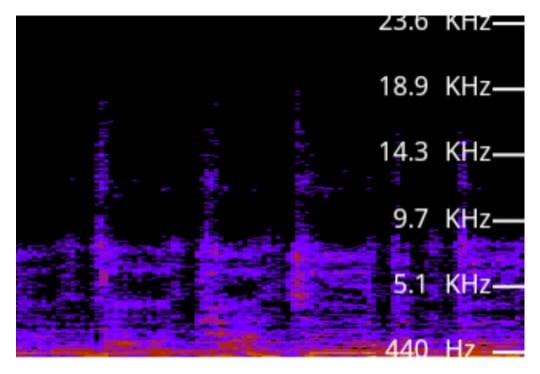
\includegraphics[width=\columnwidth]{Waveform.jpg}
\end{center}
\captionof{Spectogram observed for input audio}	
\end{figure}
\begin{figure}[!ht]
\begin{center}
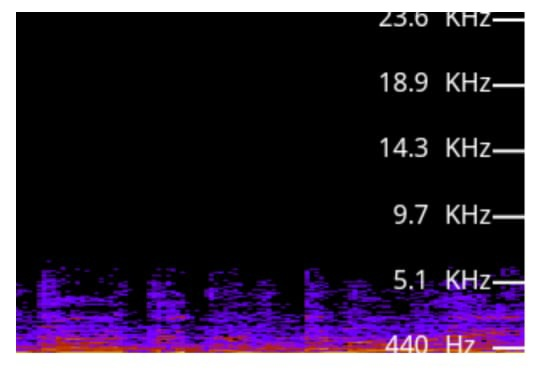
\includegraphics[width=\columnwidth]{Filtered_waveform.jpg}
\end{center}
\captionof{Spectogram observed for filtered audio}
\label{fig:xnyn}	
\end{figure}
\end{enumerate}
\section{Difference Equation}
\begin{enumerate}[label=\thesection.\arabic*,ref=\thesection.\theenumi]
\item Let
\begin{equation}
x(n) = \cbrak{\underset{\uparrow}{1},2,3,4,2,1}
\end{equation}
c \item Let
\begin{multline}
\label{eq:iir_filter}
y(n) + \frac{1}{2}y(n-1) = x(n) + x(n-2), 
\\
 y(n) = 0, n < 0
\end{multline}
Sketch $y(n)$.
\\
\solution The following code yields Fig. \ref{fig:xnyn}.
\begin{lstlisting}
https://github.com/Kaustubh-32/EE1205-Assignments/blob/main/Audio_Processing/codes/2_1_1.py
\end{lstlisting}
The values used were generaed by the code
\begin{lstlisting}
    https://github.com/Kaustubh-32/EE1205-Assignments/blob/main/Audio_Processing/codes/2_1_1.c
\end{lstlisting}
\begin{figure}[!ht]
\begin{center}
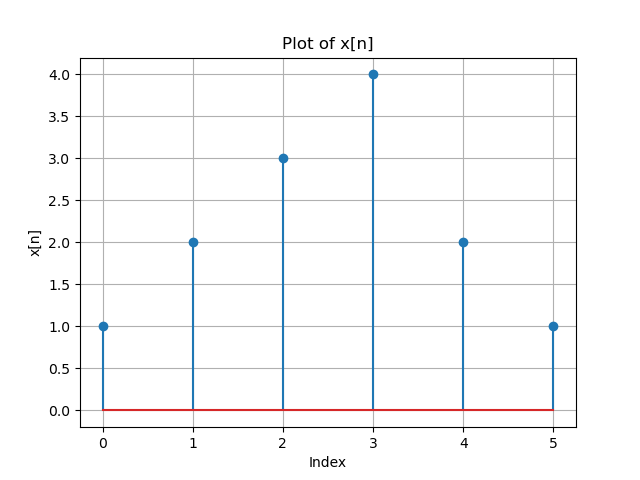
\includegraphics[width=\columnwidth]{2_1_1.png}
\end{center}
\captionof{Plot for x(n)}
\label{fig:xnyn}	
\end{figure}

The following code yields Fig. \ref{fig:xnyn1}.
\begin{lstlisting}
https://github.com/Kaustubh-32/EE1205-Assignments/blob/main/Audio_Processing/codes/2_1_2.py
\end{lstlisting}
The values used were generaed by the code
\begin{lstlisting}
    https://github.com/Kaustubh-32/EE1205-Assignments/blob/main/Audio_Processing/codes/2_1_2.c
\end{lstlisting}
\begin{figure}[!ht]
\begin{center}
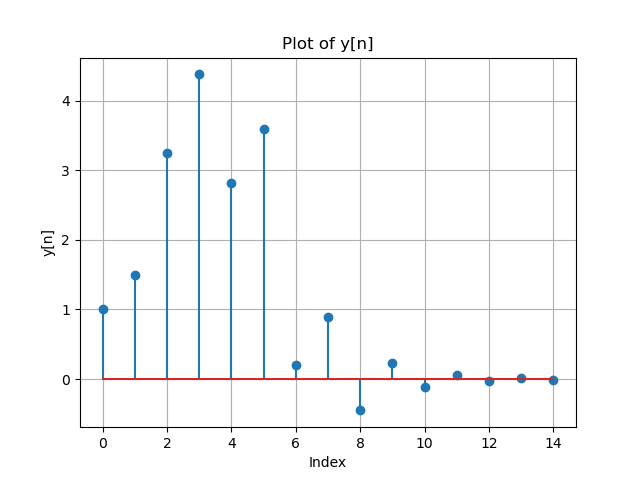
\includegraphics[width=\columnwidth]{2_1_2.png}
\end{center}
\captionof{Plot for x(n)}
\label{fig:xnyn1}	
\end{figure}
\end{enumerate}
\section{Z-transform}
\begin{enumerate}[label=\thesection.\arabic*]
\item The Z-transform of x\brak{n} is defined as
%
\begin{align}
\label{eq:eq1}
X(z)={\mathcal {Z}}\{x(n)\}=\sum _{n=-\infty }^{\infty }x(n)z^{-n}
\end{align}
%
Show that
\begin{align}
\label{eq:eq2}
{\mathcal {Z}}\{x(n-1)\} = z^{-1}X(z)
\end{align}
and find
\begin{align}
	{\mathcal {Z}}\{x(n-k)\} 
\end{align}
\solution From \eqref{eq:eq1},
\begin{align}
{\mathcal {Z}}\{x(n-k)\} &=\sum _{n=-\infty }^{\infty }x(n-1)z^{-n}\\
&=\sum _{n=-\infty }^{\infty }x(n)z^{-n-1} = z^{-1}\sum _{n=-\infty }^{\infty }x(n)z^{-n}
\end{align}
resulting in \eqref{eq:eq2}. Similarly, it can be shown that
%
\begin{equation}
\label{eq:z_trans_shift}
	{\mathcal {Z}}\{x(n-k)\} = z^{-k}X(z)
\end{equation}

\item Find
%
\begin{equation}
H(z) = \frac{Y(z)}{X(z)}
\end{equation}
%
from  \eqref{eq:iir_filter} assuming that the $Z$-transform is a linear operation.
\\
\solution  Applying \eqref{eq:z_trans_shift} in \eqref{eq:iir_filter},
\begin{align}
Y(z) + \frac{1}{2}z^{-1}Y(z) &= X(z)+z^{-2}X(z)
\\
\implies \frac{Y(z)}{X(z)} &= \frac{1 + z^{-2}}{1 + \frac{1}{2}z^{-1}}
\label{eq:freq_resp}
\end{align}
%
\item Find the Z transform of 
\begin{equation}
\delta(n)
=
\begin{cases}
1 & n = 0
\\
0 & \text{otherwise}
\end{cases}
\end{equation}
and show that the $Z$-transform of
\begin{equation}
\label{eq:unit_step}
u(n)
=
\begin{cases}
1 & n \ge 0
\\
0 & \text{otherwise}
\end{cases}
\end{equation}
is
\begin{equation}
U(z) = \frac{1}{1-z^{-1}}, \quad \abs{z} > 1
\end{equation}
\solution It is easy to show that
\begin{equation}
\delta(n) \system{Z} 1
\end{equation}
and from \eqref{eq:unit_step},
\begin{align}
U(z) &= \sum _{n= 0}^{\infty}z^{-n}
\\
&=\frac{1}{1-z^{-1}}, \quad \abs{z} > 1
\end{align}
using the formula for the sum of an infinite geometric progression.
%
\item Show that 
\begin{equation}
\label{eq:anun}
a^nu(n) \system{Z} \frac{1}{1-az^{-1}} \quad \abs{z} > \abs{a}
\end{equation}
\solution 
\begin{align}
	a^nu(n) &\system{Z} \sum_{n = 0}^{\infty}\brak{az^{-1}}^n \\
			&= \frac{1}{1-az^{-1}} \quad \abs{z} > \abs{a}
\end{align}
%
\item 
Let
\begin{equation}
H\brak{e^{\j \omega}} = H\brak{z = e^{\j \omega}}.
\end{equation}
Plot $\abs{H\brak{e^{\j \omega}}}$.  Comment.  $H(e^{\j \omega})$ is
known as the {\em Discret Time Fourier Transform} (DTFT) of $x(n)$.
\\
\solution The following code plots the magnitude of transfer function.
\begin{lstlisting}
    https://github.com/Kaustubh-32/EE1205-Assignments/blob/main/Audio_Processing/codes/3_5.py
\end{lstlisting}

\begin{figure}[H]
\centering
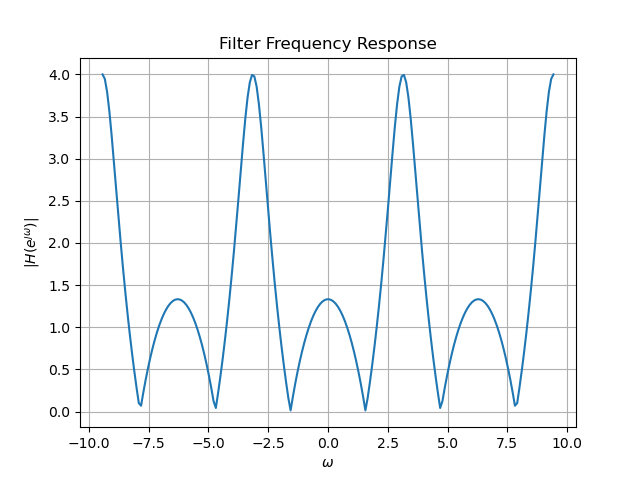
\includegraphics[width=\columnwidth]{3_5.png}
\caption{$\abs{H\brak{e^{j\omega}}}$}
\label{fig:H(z)_3.5}
\end{figure}
\end{enumerate}

\section{Impulse Response}
\begin{enumerate}[label=\thesection.\arabic*]
\item \label{prob:impulse_resp}
Find an expression for $h(n)$ using $H(z)$, given that 
%in Problem \ref{eq:ztransab} and \eqref{eq:anun}, given that
\begin{equation}
\label{eq:impulse_resp}
h(n) \system{Z} H(z)
\end{equation}
and there is a one to one relationship between $h(n)$ and $H(z)$. $h(n)$ is known as the {\em impulse response} of the
system defined by \eqref{eq:iir_filter}.
\\
\solution From \eqref{eq:freq_resp},
\begin{align}
H(z) &= \frac{1}{1 + \frac{1}{2}z^{-1}} + \frac{ z^{-2}}{1 + \frac{1}{2}z^{-1}}
\\
\implies h(n) &= \brak{-\frac{1}{2}}^{n}u(n) + \brak{-\frac{1}{2}}^{n-2}u(n-2)\label{eq:eq_h}
\end{align}
using \eqref{eq:anun} and \eqref{eq:z_trans_shift}.
\item Sketch $h(n)$. Is it bounded? Convergent? 
\\
\solution The following code plots Fig. \ref{fig:hn}.
\begin{lstlisting}
https://github.com/Kaustubh-32/EE1205-Assignments/blob/main/Audio_Processing/codes/4_2.py
\end{lstlisting}
\begin{figure}[!ht]
\centering
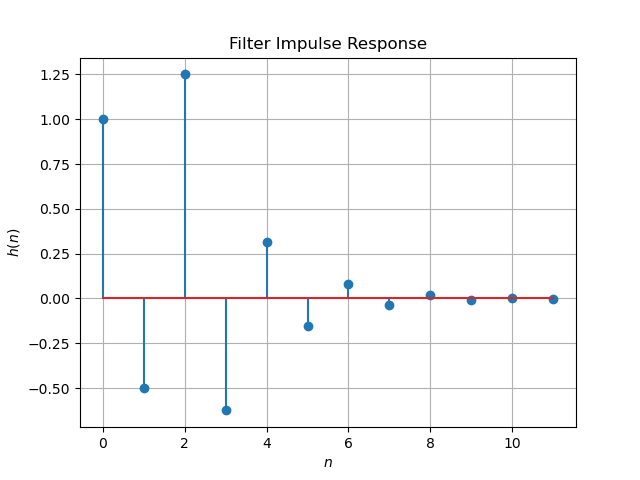
\includegraphics[width=\columnwidth]{4_2.png}
\caption{$h(n)$ as the inverse of $H(z)$}
\label{fig:hn}
\end{figure}
%
\item The system with $h(n)$ is defined to be stable if
\begin{equation}
\sum_{n=-\infty}^{\infty}h(n) < \infty
\end{equation}
Is the system defined by \eqref{eq:iir_filter} stable for the impulse response in \eqref{eq:impulse_resp}?

\solution \\
By equation \eqref{eq:eq_h},
\begin{align}
h(n) &= \brak{-\frac{1}{2}}^{n}u(n) + \brak{-\frac{1}{2}}^{n-2}u(n-2)\\
   \implies \lim_{n \to \infty} h(n) &= 0 \label{eq:eqA4.3}
\end{align}
We got to equation \eqref{eq:eqA4.3} as u(n) and u(n-2) are 1 for the limit and as $|-\frac{1}{2}| < 1$ due to which it raised to very large n will be 0.

Thus, as  $lim_{n \to \infty} h(n) = 0$, we can say that h(n) will converge.

Hence, \begin{equation}
\sum_{n=-\infty}^{\infty}h(n) < \infty
\end{equation}
As it converges, it is stable.

\item 
Compute and sketch $h(n)$ using 
\begin{equation}
\label{eq:iir_filter_h}
h(n) + \frac{1}{2}h(n-1) = \delta(n) + \delta(n-2), 
\end{equation}
\solution

%
This is the definition of $h(n)$.
\\
\solution The following code plots Fig. \ref{fig:hndef}. Note that this is the same as Fig. 
\ref{fig:hn}. 
%
\begin{lstlisting}
https://github.com/Kaustubh-32/EE1205-Assignments/blob/main/Audio_Processing/codes/4_4.py
\end{lstlisting}
\begin{figure}[!ht]
\centering
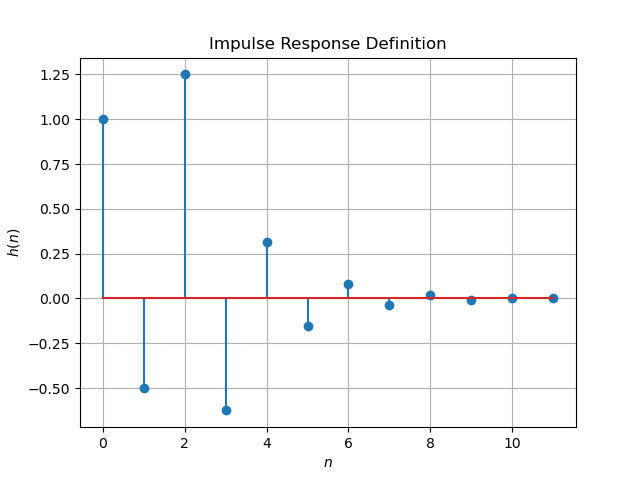
\includegraphics[width=\columnwidth]{hndef4_4.png}
\caption{$h(n)$ from the definition}
\label{fig:hndef}
\end{figure}
%
\item Compute 
%
\begin{equation}
\label{eq:convolution}
y(n) = x(n)*h(n) = \sum_{n=-\infty}^{\infty}x(k)h(n-k)
\end{equation}
%
Comment. The operation in \eqref{eq:convolution} is known as
{\em convolution}.
%
\\
\solution The following code plots Fig. \ref{fig:ynconv}. Note that this is the same as 
$y(n)$ in  Fig. 
\ref{fig:xnyn}. 
%
\begin{lstlisting}
https://github.com/Kaustubh-32/EE1205-Assignments/blob/main/Audio_Processing/codes/4_5.py
\end{lstlisting}
\begin{figure}[!ht]
\centering
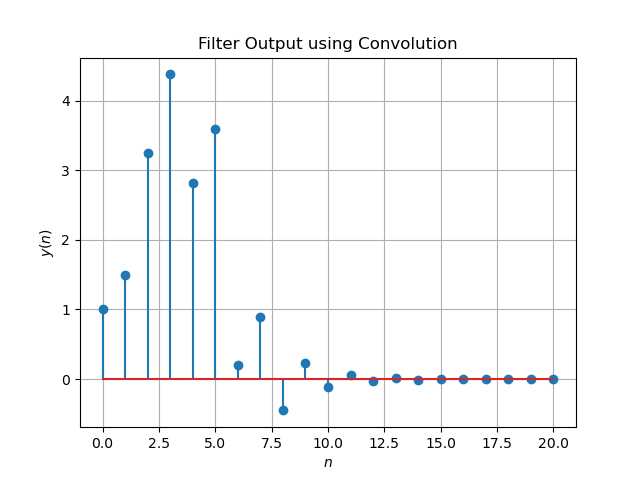
\includegraphics[width=\columnwidth]{4_5.png}
\caption{$y(n)$ from the definition of convolution}
\label{fig:ynconv}
\end{figure}

\item Show that
\begin{equation}
y(n) =  \sum_{k=-\infty}^{\infty}x(n-k)h(k)
\end{equation}
\solution
In \eqref{eq:convolution}, we substitute $r = n - k$ to get
\begin{align}
y\brak{n} &= \sum_{r=-\infty}^{\infty}x\brak{r}h\brak{n - r} \\
		  &= \sum_{n - r=-\infty}^{\infty}x\brak{n - r}h\brak{r} \\
		  &= \sum_{r=-\infty}^{\infty}x\brak{n - r}h\brak{r}
\end{align}

\end{enumerate}

%
\section{DFT and FFT}
\begin{enumerate}[label=\thesection.\arabic*]
\item
Compute
\begin{equation}
X(k) \define \sum _{n=0}^{N-1}x(n) e^{-\j2\pi kn/N}, \quad k = 0,1,\dots, N-1
\end{equation}
and $H(k)$ using $h(n)$.
\item Compute 
\begin{equation}
Y(k) = X(k)H(k)\label{eq:eq_Y}
\end{equation}
\item Compute
\begin{equation}
 y\brak{n}={\frac {1}{N}}\sum _{k=0}^{N-1}Y\brak{k}\cdot e^{\j 2\pi kn/N},\quad n = 0,1,\dots, N-1
\end{equation}
\\
\solution The following code plots Fig. \ref{fig:ynconv}. Note that this is the same as 
$y(n)$ in  Fig. 
\ref{fig:xnyn}. 
%
\begin{lstlisting}
https://github.com/Kaustubh-32/EE1205-Assignments/blob/main/Audio_Processing/codes/5_123.py
\end{lstlisting}
\begin{figure}[!ht]
\centering
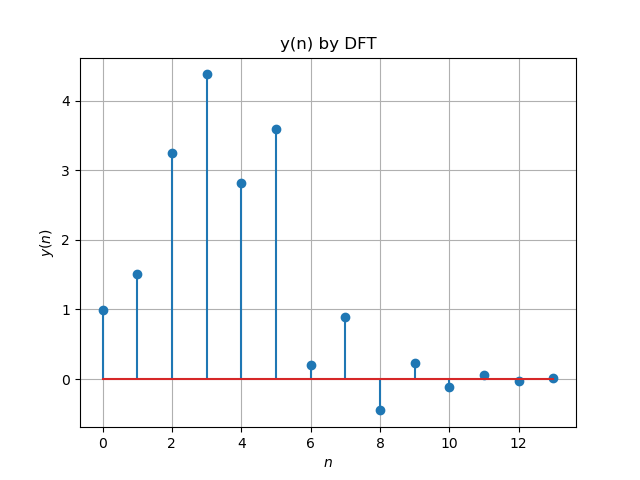
\includegraphics[width=\columnwidth]{5_123.png}
\caption{$y(n)$ from the DFT}
\label{fig:yndft}
\end{figure}

\item Repeat the previous exercise by computing $X(k), H(k)$ and $y(n)$ through FFT and 
IFFT.\\
\solution \\
The above exercise has been performed in the code below
\begin{lstlisting}
    https://github.com/Kaustubh-32/EE1205-Assignments/blob/main/Audio_Processing/codes/5_4.py
\end{lstlisting}
\begin{figure}[!ht]
\centering
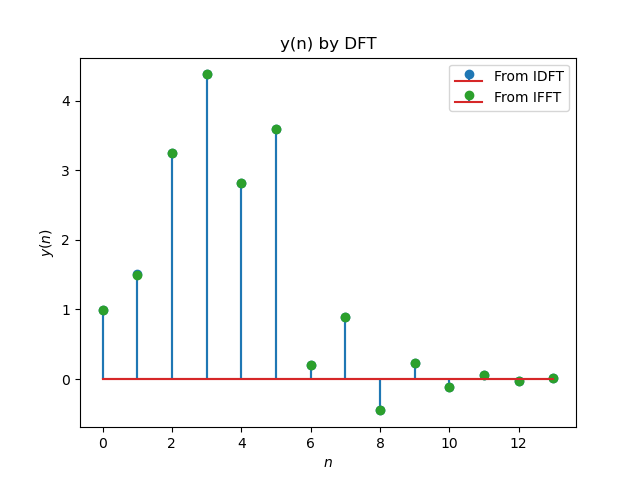
\includegraphics[width=\columnwidth]{yn_verf_5_4.png}
\caption{$y(n)$ from the FFT abd IFFT}
\label{fig:yndft}
\end{figure}
\item Wherever possible, express all the above equations as matrix equations.

\solution
Any DFT equation can be written as
\begin{align}
    \mtx{X} = \mtx{W}\mtx{x}
\end{align}
Where matrix W is given by 
\begin{align}
	\mtx{W} = 
	\begin{pmatrix}
		\omega^0 & \omega^0 & \ldots & \omega^0 \\
		\omega^0 & \omega^1 & \ldots & \omega^{N - 1} \\
		\vdots & \vdots & \ddots & \vdots \\
		\omega^0 & \omega^{N - 1} & \ldots & \omega^{(N -1)(N - 1)}
	\end{pmatrix}
\end{align}
 $\omega=e^{-\frac{j2\pi}{N}}$ 
 \begin{align}
	\mtx{X} = 
	\begin{pmatrix}
		X(0) \\ X(1) \\ \vdots \\ X(n - 1)
	\end{pmatrix}
\end{align}
Thus we can rewrite  \eqref{eq:eq_Y} as:
\begin{align}
	\mtx{Y} = \mtx{X}\odot\mtx{H} = \brak{\mtx{W}\mtx{x}}\odot\brak{\mtx{W}\mtx{h}}
\end{align}
$\odot$ is the element-wise multiplication of the matrices (Hadamard product).

\end{enumerate}
%
\section{Exercises}

Answer the following questions by looking at the python code in Problem \ref{prob:output}.
\begin{enumerate}[label=\thesection.\arabic*]
\item
The command
\begin{lstlisting}
	output_signal = signal.lfilter(b, a, input_signal)
	\end{lstlisting}
in Problem \ref{prob:output} is executed through the following difference equation
\begin{equation}
\label{eq:iir_filter_gen}
 \sum _{m=0}^{M}a\brak{m}y\brak{n-m}=\sum _{k=0}^{N}b\brak{k}x\brak{n-k}
\end{equation}
%
where the input signal is $x(n)$ and the output signal is $y(n)$ with initial values all 0. Replace
\textbf{signal.filtfilt} with your own routine and verify.
%
\solution\\
The following code defines a custom signal.filtfilt function :
\begin{lstlisting}
    https://github.com/Kaustubh-32/EE1205-Assignments/blob/main/Audio_Processing/codes/6_1.py
\end{lstlisting}
\begin{figure}[!ht]
\centering
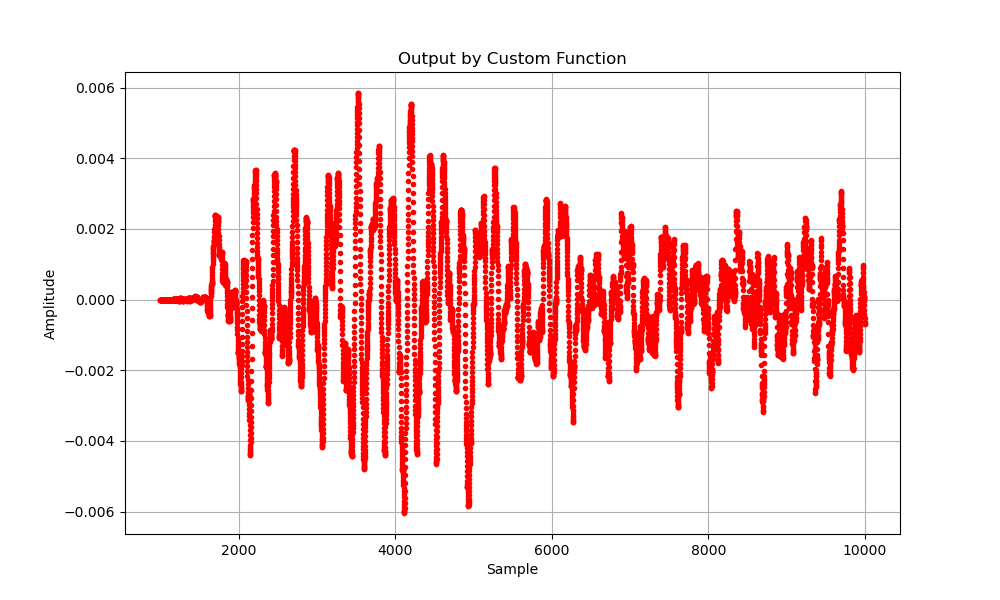
\includegraphics[width=\columnwidth]{output_custom.png}
\caption{Plot using my routine for signal.filtfilt}
\label{fig:ff1}
\end{figure}
\begin{figure}[!ht]
\centering
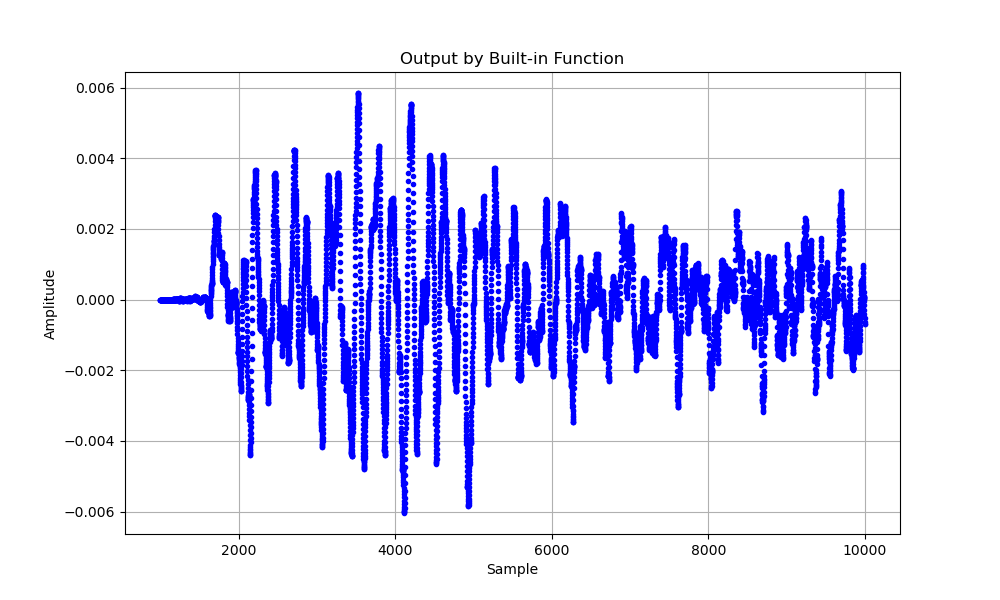
\includegraphics[width=\columnwidth]{output_builtin.png}
\caption{Plot using builtin function}
\label{fig:ff2}
\end{figure}



\item Repeat all the exercises in the previous sections for the above $a$ and $b$.

\solution
\begin{align}
    M &= 5\\
    N&=5
\end{align}
a = 1 , -2.15448443 , 1.98942448 , -0.86509739 , 0.14814218\\


b = 0.00737405 , 0.02949621 , 0.04424432 , 0.02949621, 0.00737405\\


\begin{align}
    &a\brak{0}y\brak{n} + a\brak{1}y\brak{n-1}+a\brak{2}y\brak{n-2}+a\brak{3}\\ \notag &y\brak{n-3} + a\brak{4}y\brak{n-4} =   b\brak{0}x\brak{n} + b\brak{1}x\brak{n-1}\\ \notag &+b\brak{2}x\brak{n-2}+b\brak{3}x\brak{n-3} + b\brak{4}x\brak{n-4} 
\end{align}
Difference Equation is given by :
\begin{align}
	&y(n) - \brak{-2.15448443}y(n - 1) + \brak{1.98942448}y(n - 2) \nonumber \\
	&- \brak{-0.86509739}y(n - 3) + \brak{ 0.14814218}y(n - 4) \nonumber \\
	&= \brak{0.00737405}x(n) + \brak{ 0.02949621}x(n - 1) \nonumber \\
	&+ \brak{0.04424432}x(n - 2) + \brak{ 0.02949621}x(n - 3) \nonumber \\
	&+ \brak{0.00737405}x(n - 4)
\end{align}
From \eqref{eq:iir_filter_gen} 
\begin{align}
    H(z) &= \frac{b_0 + b_1 z^{-1} + b_2 z^{-2} + \ldots + b_M z^{-N}}{a_0 + a_1 z^{-1} + a_2 z^{-2} + \ldots + a_N z^{-M}}\\
    H(z) &= \frac{\sum_{k = 0}^{N}b(k)z^{-k}}{\sum_{k = 0}^{M}a(k)z^{-k}} \label{eq:trans-func}
\end{align}
Partial fraction on \eqref{eq:trans-func} can be generalised as:
\begin{align}
    H\brak{z}&= \sum_{i}\frac{r(i)}{1 - p(i)z^{-1}} + \sum_{j}k(j)z^{-j}
	\label{eq:trans-func-pfe}
\end{align}
Now,
\begin{align}
    a^{n}u\brak{n} \system{Z} \frac{1}{1-az^{-1}} \label{eq:res-1}\\
    \delta\brak{n-k} \system{Z} z^{-k}\label{eq:res-2}
\end{align}
Taking inverse z transform of \eqref{eq:trans-func-pfe} by using \eqref{eq:res-1} and \eqref{eq:res-2}
\begin{align}
h(n) &= \sum_{i}r(i)[p(i)]^nu(n) + \sum_{j}k(j)\delta(n - j)
	\label{eq:h-n-expr}
\end{align}
The below code computes the values of $r\brak{i},p\brak{i} , k\brak{i}$ and plots $h\brak{n}$
\begin{lstlisting}
https://github.com/Kaustubh-32/EE1205-Assignments/blob/main/Audio_Processing/codes/6_2_2_hn.py
\end{lstlisting}
%\input{tables/audio_filter_tab}

\textbf{Stability of h(n)}:\\
\begin{align}
H\brak{z} &= \sum_{n = 0}^{\infty} h\brak{n}z^{-n}\\
H(1)&= \sum_{n = 0}^{\infty}h(n)  = \frac{\sum_{k = 0}^{N}b(k)}{\sum_{k = 0}^{M}a(k)}< \infty
\end{align}
As both $a\brak{k}$ and $b\brak{k}$ are finite length sequences they converge.\\
The below code plots Filter frequency response
\begin{lstlisting}
https://github.com/Kaustubh-32/EE1205-Assignments/blob/main/Audio_Processing/codes/6_2_3.py
\end{lstlisting}
\begin{figure}[H]
\centering
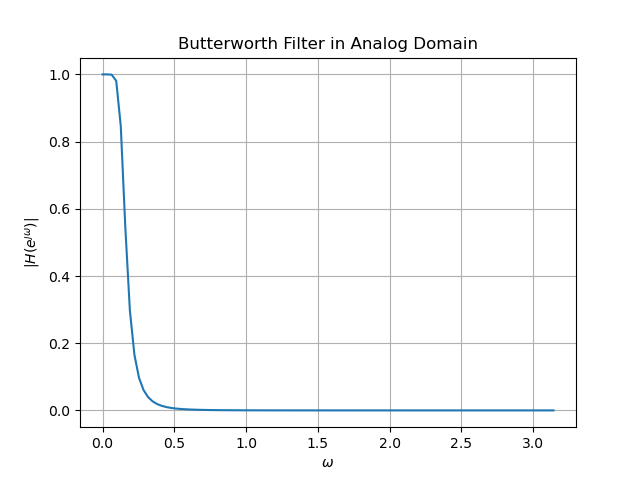
\includegraphics[width=1\columnwidth]{6_2_3.png}
\caption{Frequency Response of Audio Filter}
\label{fig:H(w)_6}
\end{figure}
The below code plots the Butterworth Filter in analog domain by using bilinear transform.
\begin{align}
    z=\frac{1+sT/2}{1-sT/2}
\end{align}
\begin{lstlisting}
https://github.com/Kaustubh-32/EE1205-Assignments/blob/main/Audio_Processing/codes/6_2_4.py
\end{lstlisting}
\begin{figure}[H]
\centering
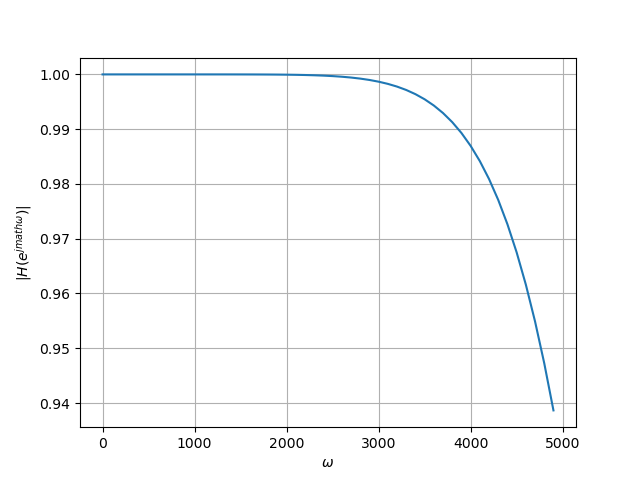
\includegraphics[width=1\columnwidth]{6_2_4.png}
\caption{Butterworth Filter Frequency response in analog domain}
\label{fig:H(w)_6}
\end{figure}



The below code plots the Pole-Zero Plot of the frequency response.
\begin{lstlisting}
https://github.com/Kaustubh-32/EE1205-Assignments/blob/main/Audio_Processing/codes/6_2_2.py
\end{lstlisting}
\begin{figure}[H]
\centering
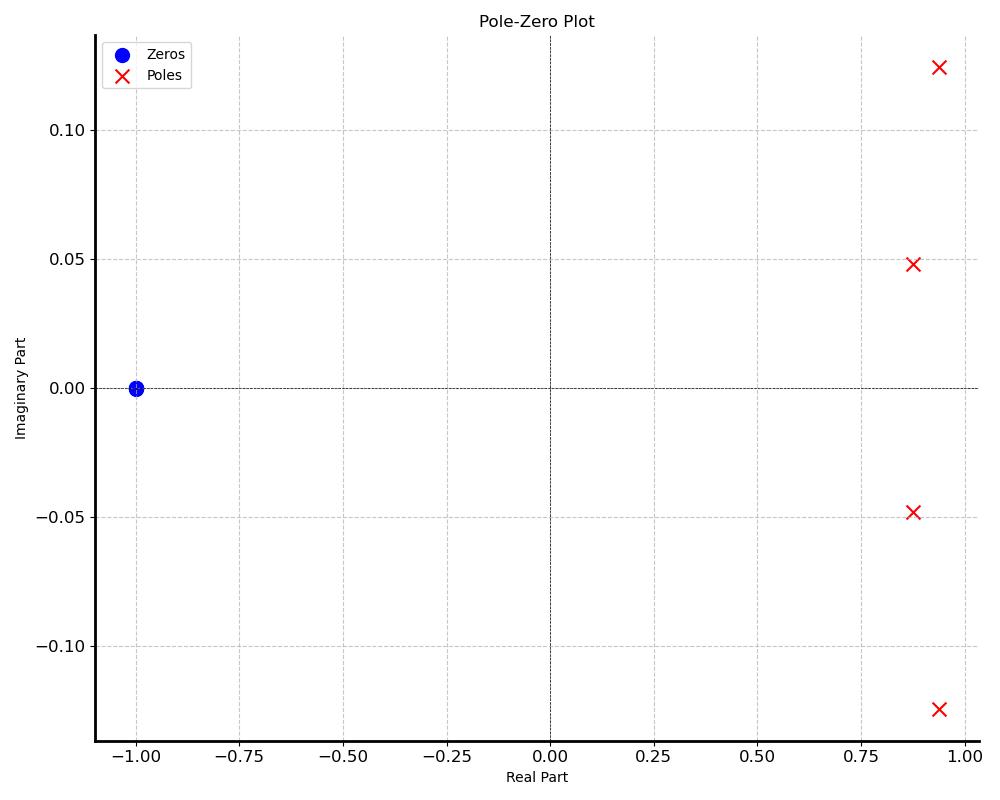
\includegraphics[width=1\columnwidth]{6_2_2_pole.png}
\caption{There are complex poles. So $h\brak{n}$ should be damped sinusoid.}
\label{fig:pole_zero_6.2}
\end{figure}

\begin{figure}[H]
\centering
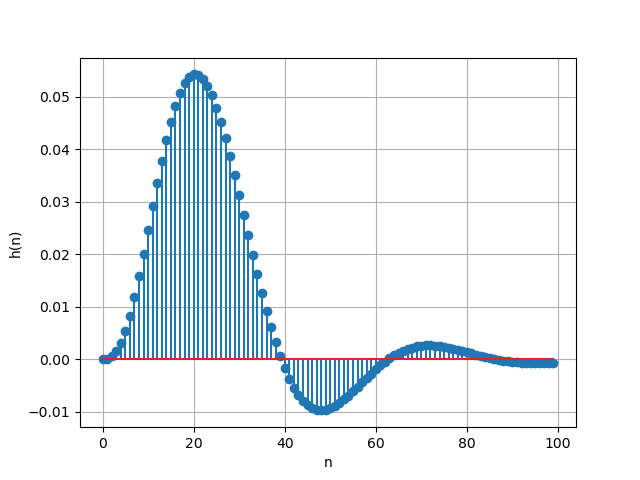
\includegraphics[width=\columnwidth]{h(n)_6.2.png}
\caption{h(n) of Audio Filter.It is a damped sinusoid.}
\label{fig:6.2_hn}
\end{figure}


\item What is the sampling frequency of the input signal?
\\
\solution\\
Sampling frequency(fs)=44.1kHZ.
\item
What is type, order and  cutoff-frequency of the above butterworth filter
\\
\solution\\
The given butterworth filter is low pass with order=2 and cutoff-frequency=4kHz.
%
\item
Modifying the code with different input parameters and to get the best possible output.
%
\solution 

The output can be improved by increasing the order of the filter. Also, the cutoff frequency can be changed to ensure undesired frequencies are filtered out.
\end{enumerate}
\end{document}
